\input{header}

\AtBeginSubsection[]
{
	\begin{frame}<beamer>
		\frametitle{Outline}
		\tableofcontents[current,currentsubsection]
	\end{frame}
}

\begin{document}


\begin{frame}[allowframebreaks]
\frametitle{$E_{\text{LBA}}$ Undecidable}
\begin{itemize}
\item We have seen that
  \begin{center}
    \begin{tabular}{l}
      $A_{\text{TM}}$ undecidable \\
      $A_{\text{LBA}}$ decidable 
    \end{tabular}
  \end{center}
\item However,
    \begin{equation*}
  E_{\text{LBA}}=
\{\langle  M\rangle\mid M \mbox{ is an LBA where } L(M) = \emptyset\}
\end{equation*}
is undecidable
\item We do the proof by the computation history method
\item Idea: the question of $M$ accepts $w$ can be solved by
  checking if $L(B) = \emptyset$, where $B$ is an LBA
\item Then because we assume $E_{\text{LBA}}$ is decidable, we have a decider
  for $A_{\text{TM}}$
\item The design of $B$: $B$ recognizes all accepting computation
  histories for $M$ on $w$
  \begin{center}
    \begin{tabular}{l}
      $M$ accepts $w \Rightarrow L(B) \neq \emptyset$\\
      $M$ rejects $w \Rightarrow L(B) = \emptyset$
    \end{tabular}
  \end{center}
\item We see that the machine is designed according to the given
  $w$. This strategy has been used in earlier examples
  
\item Details of $B$: on any input $x$, we check if $x$ is an
  accepting computation history for $M$ on $w$
\item Specifically, we check if $x$ is
  \begin{equation}
    \#\underbrace{\qquad}_{C_1}\#\underbrace{\qquad}_{C_2}\#\cdots\#\underbrace{\qquad}_{C_l}\#
    \label{eq:C1toCl}
  \end{equation}
  and $C_1, \ldots, C_l$ satisfy that
  \begin{center}
  \begin{tabular}{l}
    $C_1$  is the start configuration,\\
    $C_l$ is an accepting configuration, and\\
    $C_i$ follows from $C_{i-1}$
  \end{tabular}
\end{center}
\item The machine looks like
  \begin{center}
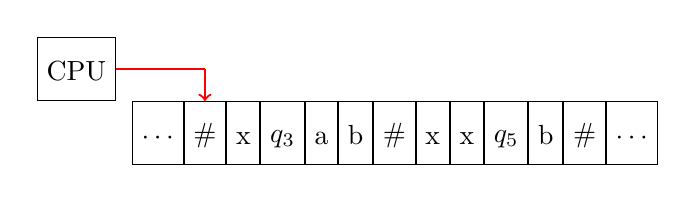
\begin{tikzpicture}[ampersand replacement=\&]
\matrix[nodes={minimum height=8mm,text height=0.3cm}] 
{
  \node[draw](0) {CPU}; \& [0.2cm] \& \node(1){}; \&\&\& \&\&\&\&\&\& \&\&\\
  \& \node[draw]{$\cdots$};
  \& \node[draw](a){\#};
  \& \node[draw]{x};
  \& \node[draw]{$q_3$};
  \& \node[draw]{a};
  \& \node[draw]{b};
  \& \node[draw]{\#};
  \& \node[draw]{x};
  \& \node[draw]{x};
  \& \node[draw]{$q_5$};
  \& \node[draw]{b};
  \& \node[draw]{\#};
  \& \node[draw]{$\cdots$};
\\
};
\draw [-,red,thick] (0) -- (1.center) ;
\draw [->,red,thick] (1.center) -- (a) ;
\end{tikzpicture}
\end{center}
\item To begin, we check if the input $x$ is in the form of
  \eqref{eq:C1toCl}
\item Next, $C_1$ is $q_0 w$, so checking the first condition is
  easy
\item For the third condition, we scan if $C_l$ contains $q_{\text{accept}}$
\item Now $C_i$ and $C_{i+1}$ are the same except around the
  head position
\item To compare $C_i$ and $C_{i+1}$, the TM zigzags between
  them

\item The setting looks good, but
  remember that $B$ is an LBA
\item The above discussion seems to show that our operations
  never go beyond $|x|$
\item On the other hand, if you think extra space is needed, it is
  fine as long as the space needed is 
  bounded by a constant factor of the
  length of $\#C_1\# \cdots \# C_l\#$
\item For example, if we copy $C_i$ and $C_{i+1}$ to
  the end for the comparison, the extra space needed is no more than
  $|\#C_1\# \cdots \# C_l\#|$
\item Thus for input $x$ we can check if the first
  half is $\#C_1\# \cdots \# C_l\#$
\item Then the machine never goes beyond $|x|$.
Further, if $M$ accepts $w$,
  then at least one $x$ is accepted by $B$
\end{itemize}
\end{frame}

\begin{frame}[allowframebreaks]
\frametitle{$ALL_{\text{CFG}}$ Undecidable}
\begin{itemize}
\item Earlier we proved that
  \begin{equation*}
  E_{\text{CFG}}
=\{\langle  G\rangle \mid
G: CFG, L(G)=\emptyset\}
\end{equation*}
is decidable
\item Now we show a related problem is undecidable
  \begin{equation*}
  ALL_{\text{CFG}}
=\{\langle  G\rangle \mid
G: CFG, L(G)=\Sigma^* \}
\end{equation*}
\item It checks if $G$ generates all possible strings
\item The proof is still by contradiction
\item[]  We assume $ALL_{\text{CFG}}$ is decidable
\item Idea: consider a CFG $G$ such that
  \begin{equation*}
    G \text{ generates } \Sigma^*
    \Leftrightarrow
    M \text{ does not accept } w
  \end{equation*}
\item This is equivalent to
  \begin{equation*}
    \begin{cases}
      G \text{ generates } \Sigma^*
      &
      \text{if } M \text{ does not accept } w \\
      G \text{ fails on some strings} 
      &
      \text{if } M \text{ accepts } w 
    \end{cases}
  \end{equation*}
\item If we have a decider on $G$, then we have
  a decider on $A_{\text{TM}}$
\item If $M$ accepts $w$, we let $G$ fail to generate
  \begin{center}
    an accepting computation history for $M$ on $w$
  \end{center}
\item That is, for $G$, the input cannot be
  \begin{equation*}
    \#\underbrace{\qquad}_{C_1}\#\underbrace{\qquad}_{C_2}\#\cdots\#\underbrace{\qquad}_{C_l}\#
  \end{equation*}
where $C_1, \ldots, C_l$ satisfy that
  \begin{center}
  \begin{tabular}{l}
    $C_1$  is the start configuration,\\
    $C_l$ is an accepting configuration, and\\
    $C_i$ follows from $C_{i-1}$
  \end{tabular}
\end{center}
\item  Therefore, $G$ generates all strings
  \begin{enumerate}
  \item that do not start with $C_1$,
  \item that do not end with an accepting configuration, \alert{or}
  \item $C_i$ does not yield $C_{i+1}$
  \end{enumerate}
\item Note that it's ``or'' because the opposite of
  \begin{equation*}
    A \text{ and } B \text{ and } C
  \end{equation*}
  is
  \begin{equation*}
    \neg A \text{ or } \neg B \text{ or } \neg C
  \end{equation*}

\item On the other hand, if $M$ does not accept $w$, no accepting computation
  history exists
\item [] Then $G$ generates all strings
\item But how to construct such a CFG?
\item Let's generate an equivalent PDA
\item The PDA nondeterministically checks three branches
  for the three requirements
\item For example, the first branch checks if the beginning
  of the input is $C_1$ and
  accepts if it is not
\item The third branch is more complicated
\item It accepts if $C_i$ does not properly yields $C_{i+1}$
\item We can push $C_i$ to stack (\# allows us to extract $C_i$)
\item We pop the stack to compare $C_i$ and $C_{i+1}$
\item They are the same except around the head position
\item A problem is that when we pop $C_i$, it is in
  the reverse order
\item To enable the comparison, we write the accepting
  computation history differently
  \begin{equation*}
    \#\underbrace{\quad \rightarrow \quad}_{C_1}\#\underbrace{\quad \leftarrow \quad}_{C_2^R}\#
    \underbrace{\quad \rightarrow \quad}_{C_3}\#\underbrace{\quad \leftarrow \quad}_{C_4^R}\#
    \cdots\#\underbrace{\qquad}_{C_l}\#
  \end{equation*}
\item By this way, when we pop $C_2^R$, we get $C_2$ and can do the
  comparison
\item This means that for any input $x$, if it is in the form of
  $\#C_1\# \cdots \# C_l\#$, we ``treat'' the second
  segment as $C_2^R$ in designing operations
\end{itemize}
\end{frame}

\end{document}

%%% Local Variables:
%%% mode: latex
%%% TeX-master: t
%%% End